\section{Additional Requirements}
	
	\subsection{Functionality}

		\subsubsection{General}
			\begin{itemize}
				\item The game will be played on the same device and \gls{GUI}.
				\item The game will be implemented to allow distributed sessions in the future.
			\end{itemize}

        \subsubsection{Game Rules}
			\textbf{Goal} \\
            The objective of the game is to be the first one to reach the finish line. If multiple players finish the race with the same amount of turns, it will result in a draw. \\
            
            \textbf{Environment} \\
            The game board is a checkered piece of paper with a track, starting line and finish line. All the grid points on the track are accessible by the players with their respective moves.
            \begin{figure}[H]
                \centering
                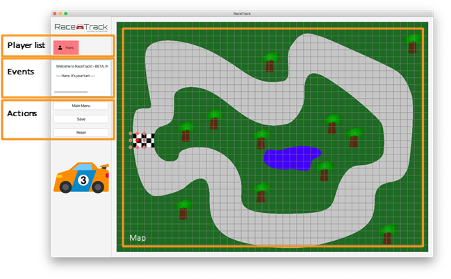
\includegraphics[width=14cm,keepaspectratio,center]{img/Additional-Requirements_Environment-Example.png}
                \caption{Example of the environment in the game}
            \end{figure}

            \textbf{The course of the game} \\
            All players start from the starting line. The first player is determined randomly. After each move of a participant, the next competitor takes his turn until every player reaches the finish line. A finished player will not be able to move again. \\

            \textbf{Moving around} \\
            Each player's first move must lead to one of the five neighbors of the starting point moving forward. On the first move, it is not possible to go backward. In each following move, the so-called base for this move is determined. The base is dependent on repeating the previous move, both horizontally and vertically. This calculation in RaceTrack is also known as velocity in the game. \\

            \newpage

            \textbf{Example} \\
            \say{If the player last moved two boxes to the right and four boxes up, the main point is now two boxes to the right and four above the current starting point. The player now can move directly to the main point or one of his eight neighbors.}
            \begin{figure}[H]
                \centering
                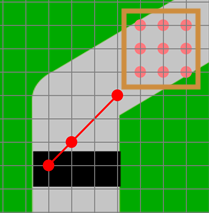
\includegraphics[width=5cm,keepaspectratio,center]{img/Additional-Requirements_Moving-Around-Example.png}
                \caption{Example of how to move around the game}
            \end{figure}

            \textbf{Conditions} \\
            The cars must stay within the track boundaries. This applies to every move. Leaving the road will lead to a crash. Depending on the selected game mode, the game will react differently to a crash. Points that are occupied by another car cannot be approached. \\

            \textbf{Game Modes and Crash Handling} \\
            There are currently \textbf{three} unique game modes available:
            \begin{itemize}
                \item \textbf{Go Kart} : \textit{Continue with minimum velocity and no acceleration until the track is reached again}:
                \begin{itemize}
                    \item The player's velocity resets.
                    \item The player does not accelerate until the track is reached again.
                \end{itemize}
                \item \textbf{Formula One} : \textit{Retire from the race}:
                \begin{itemize}
                    \item The player crashes and receives a corresponding notification about it.
                    \item The player retires from the race and will not be able to do any more moves during this game session.
                \end{itemize}
                \item \textbf{Bobby Car} : \textit{Reset position to last valid point and reset velocity}:
                \begin{itemize}
                    \item The player crashes and receives a corresponding notification about it.
                    \item The player's velocity resets.
                    \item The player's car resets to his last valid position on the track.
                \end{itemize}
            \end{itemize}

        \subsubsection{Special Requirements}
            Custom tracks to be loaded into the game (UC13) need to comply with following requirements:
            \begin{itemize}
                \item The image must only consist of following colors \textit{(can still be changed during development)}:
                \begin{itemize}
                    \item \textcolor{gray}{\#C5C5C5} : represents the drivable track.
                    \item \textcolor{black}{\#000000} / \colorbox{black}{\textcolor{white}{\#FFFFFF}} : represents the starting/finish line.
                    \item Every other color will be interpreted as not to be part of the drivable track (out of track boundaries).
                \end{itemize}
                \item The starting/finish line must be placed either vertically or horizontally, it cannot be placed diagonally.
            \end{itemize}

    \subsection{Usability}
        RaceTrack's GUI must implement the fundamental concepts of usability to ensure great user experience. The following requirements are defined:
        \begin{itemize}
            \item Minimalistic GUI:
            \begin{itemize}
                \item No buttons to steer the car, only mouse clicks needed.
                \item A map to show:
                \begin{itemize}
                    \item The grid paper.
                    \item The Track.
                    \item Starting/Finish line.
                \end{itemize}
                \item A list with all current players.
                \item An event log where all past actions can be retracted.
            \end{itemize}
            \item Target interaction components should be large enough for users to both discern what it is and to accurately select them.
            \begin{itemize}
                \item minimum of 24 Pixels in width and height for buttons.
            \end{itemize}
        \end{itemize}

    \subsection{Reliability}
        The following reliability requirements are defined for RaceTrack:
        \begin{itemize}
            \item Reliability: Game breaking errors should occur at maximum once every 20 game sessions (during the Beta phase).
            \item Failure definition: A game-breaking error is a session of RaceTrack which was interrupted by a crash of the application.
        \end{itemize}

    \subsection{Performance}
        Due to the simple architecture of the application, no special performance requirements are defined. Notice the usability requirement number four, which requires the response time for user feedback to be at \textit{normal} levels (< 1s).

    \subsection{Supportability}
        Serviceability requirements:
        \begin{enumerate}
            \item The Java code must be documented.
            \item Clean code concepts will be integrated when developing RaceTrack (See PDF \textit{PROG1 Clean-Code-Regeln}).
            \item RaceTrack is developed using the \href{https://semver.org/}{Semantic Versioning specification}.
        \end{enumerate}

    \subsection{Scalability}
        There are no special requirements for scalability.
